\section{Properties of Power Spectral Density (PSD)}

\subsection*{Approximation in the definition of PSD}

Equivalence is shown by starting from equation (9), as indicated in the coursework instructions.

\begin{align}
P(w)    & = \lim_{N\to\infty} \E \bigg\{ \frac{1}{N} \bigg| \sum_{n=0}^{N-1} x(n) e^{-jwn} \bigg|^{2} \bigg\}
            \label{proof:periodogram:starter}\\
        & = \lim_{N\to\infty} \E \bigg\{\frac{1}{N}
            \sum_{m=0}^{N-1} x(m) e^{-jwm} \sum_{k=0}^{N-1} x^{*}(k) e^{jwk} \bigg\}\nonumber\\
        & = \lim_{N\to\infty} \frac{1}{N}
            \sum_{m=0}^{N-1} \sum_{k=0}^{N-1} \E \bigg\{ x(m) e^{-jwm} x^{*}(k) e^{jwk} \bigg\}\nonumber\\
        & = \lim_{N\to\infty} \frac{1}{N}
            \sum_{m=0}^{N-1} \sum_{k=0}^{N-1} \E \bigg\{ x(m) x^{*}(k) \bigg\} e^{-jw(m-k)} \nonumber\\
        & = \lim_{N\to\infty} \frac{1}{N}
            \sum_{m=0}^{N-1} \sum_{k=0}^{N-1} r_{xx}(m-k) e^{-jw(m-k)}
          = \lim_{N\to\infty} \frac{1}{N}
            \sum_{m=0}^{N-1} \sum_{k=0}^{N-1} g(m-k)
\label{proof:periodogram}
\end{align}
%
where $g(\tau) = r_{xx}(\tau) e^{-jw\tau}$. Converting the double into a single summation according to:
%
\begin{equation}
    \sum_{m=-N}^{N} \sum_{k=-N}^{N} g(m-k) = \sum_{\tau=-2N}^{2N}(2N + 1 - |\tau|)g(\tau)
\label{proof:periodogram:helper}
\end{equation}
%
(\ref{proof:periodogram}) can be written as:
%
\begin{align}
P(w)    & =         \lim_{N\to\infty} \frac{1}{N} \sum_{\tau=-(N-1)}^{N-1}(N - |\tau|)r_{xx}(\tau) e^{-jw\tau}\nonumber\\
        & =         \lim_{N\to\infty} \sum_{\tau=-(N-1)}^{N-1} r_{xx}(\tau) e^{-jw\tau} -
                    \lim_{N\to\infty} \frac{1}{N} |\tau| \sum_{\tau=-(N-1)}^{N-1} r_{xx}(\tau) e^{-jw\tau}\nonumber\\
        & \approx   \sum_{\tau=-\infty}^{\infty} r_{xx}(\tau) e^{-jw\tau}
\label{proof:periodogram:shown}
\end{align}
%
where the last equality in (\ref{proof:periodogram:shown}) is obtained under the mild assumption that the
covariance sequence $r_{xx}(k)$ decays rapidly, or equivalently:
%
\begin{equation}
    \lim_{N\to\infty} \frac{1}{N} \sum_{\tau=-(N-1)}^{N-1} |\tau| |r_{xx}(\tau)| = 0
\label{proof:periodogram:decaying-covariance}
\end{equation}
%
Thus under the mild assumption that the covariance sequence decays rapidly we have shown that (\ref{proof:periodogram:starter})
is equal to (\ref{proof:periodogram:shown}), which is the DTFT of the autocovariance function (ACF).
%
\begin{equation}
    P(w) = \sum_{t=-\infty}^{\infty} r_{xx}(t) e^{-jwt}
\end{equation}

\begin{enumerate}[label=\alph*), leftmargin=*]
%% a)
\item
%

Power Spectrum Estimation is performed by taking the Fourier Transform of the ACF, $r_{xx}(k)$. Due to the even symmetry of ACF,
its Fourier Transform, $P(w)$, is expected to be purely real, as well as non-negative since the positive semi-definiteness of the
covariance matrix, $xx^{T}$. These properties are preserved after zero-padding in the middle of the ACF, around zero, while at the
same time, frequency resolution is increased. Figure \ref{fig:1_2_a} verifies our claims in the case of the rectangular window signal,
whose width is controlled by varying $M$. Unsurprisingly, the increase of $M$ from $10$ to $128$ results in an increase of the rectangular
width and and inversely proportional decrease in the width of the mainlobe (frequency domain), while the power concentration is increased
around 0.

\begin{figure}[h]
    \centering
    \begin{subfigure}{0.49\textwidth}
        \centering
        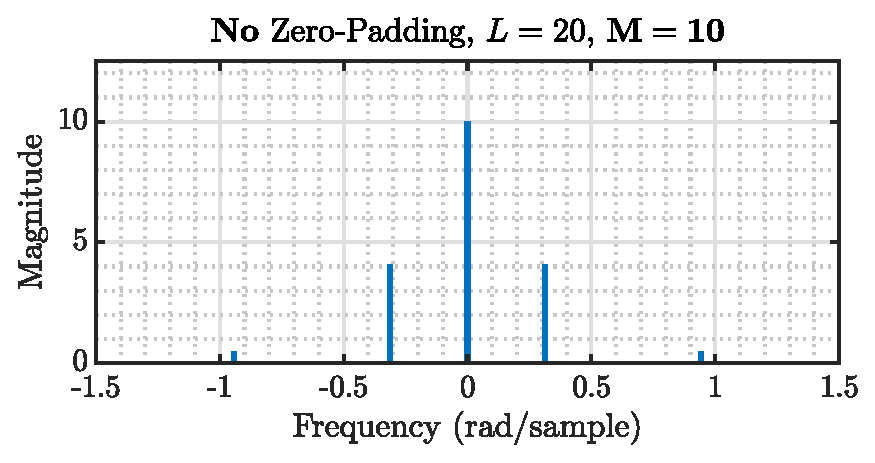
\includegraphics[height=1.5in]{report/spectrum-estimation/properties-of-power-spectral-density/assets/a/zero-pad-L_20-M_10}
    \end{subfigure}
    ~ 
    \begin{subfigure}{0.49\textwidth}
        \centering
        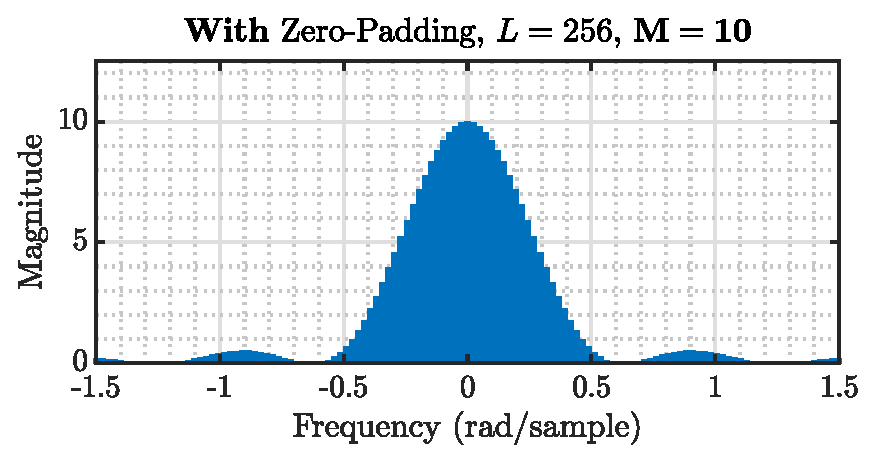
\includegraphics[height=1.5in]{report/spectrum-estimation/properties-of-power-spectral-density/assets/a/zero-pad-L_256-M_10}
    \end{subfigure}
    ~
    ~
    \begin{subfigure}{0.49\textwidth}
        \centering
        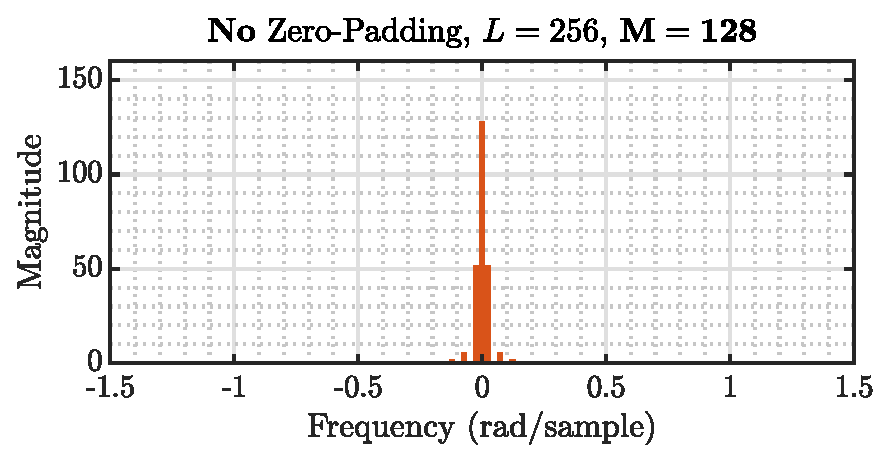
\includegraphics[height=1.5in]{report/spectrum-estimation/properties-of-power-spectral-density/assets/a/zero-pad-L_256-M_128}
    \end{subfigure}
    ~
    \begin{subfigure}{0.49\textwidth}
        \centering
        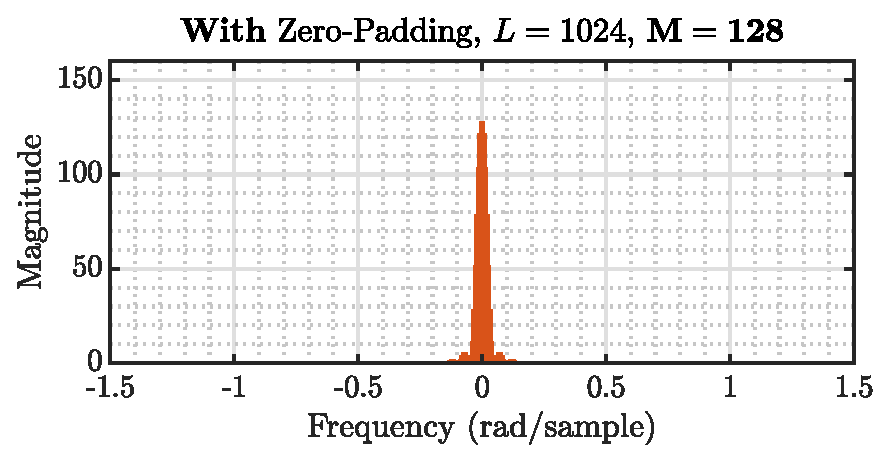
\includegraphics[height=1.5in]{report/spectrum-estimation/properties-of-power-spectral-density/assets/a/zero-pad-L_1024-M_128}
    \end{subfigure}
    \caption{Spectrum estimation using symmetric ACF and zero-padding effect.}
    \label{fig:1_2_a}
\end{figure}

%% b)
\item
%

Because of the symmetry of ACF, $P(w)$ is expected to be purely real. Nonetheless, the numerical methods used for the implementation
of \texttt{fft} and the finite precision using in computers (64-bits in this case) lead to round-off errors, introducing a negligible
imaginary part \texttt{imag(xf)}. Figure \ref{fig:1_2_b_1} demonstrates this point, verifying how trivial (16 orders of magnitude smaller)
the imaginary part is, compared to the real part, \texttt{real(xf)}, while figure \ref{fig:1_2_b_2} depicts the PSD estimates with and
without the imaginary part.

\begin{figure}[h]
    \centering
    \begin{subfigure}{0.49\textwidth}
        \centering
        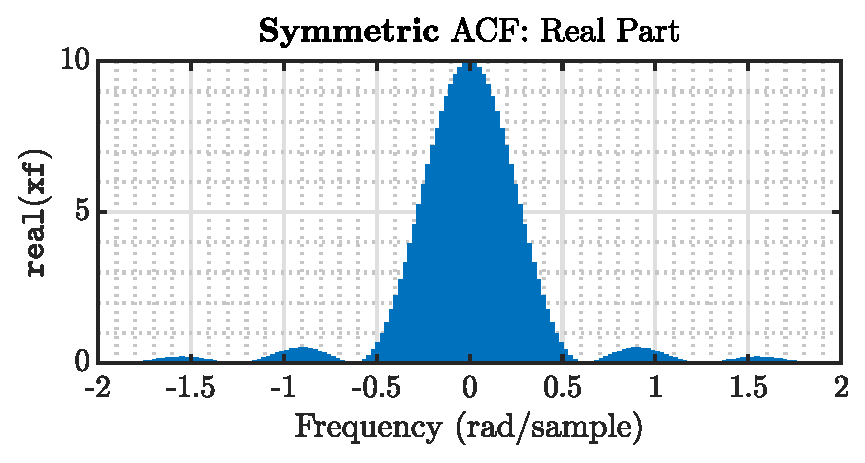
\includegraphics[height=1.5in]{report/spectrum-estimation/properties-of-power-spectral-density/assets/b/symmetric_real-M_10}
    \end{subfigure}
    ~ 
    \begin{subfigure}{0.49\textwidth}
        \centering
        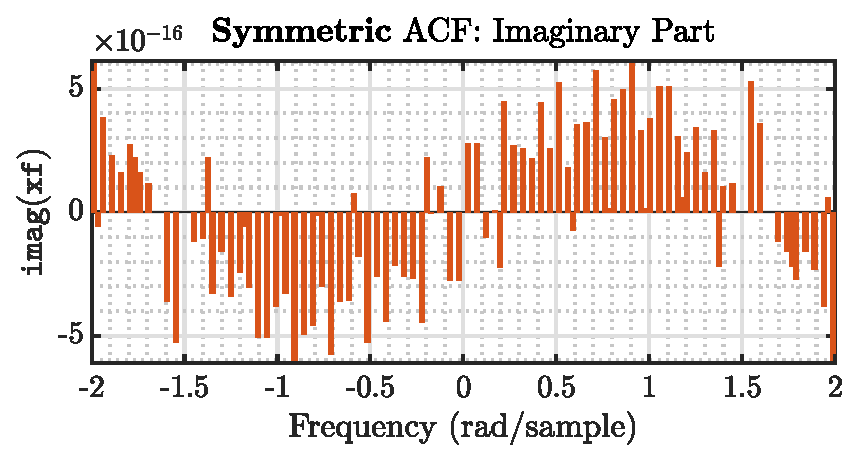
\includegraphics[height=1.5in]{report/spectrum-estimation/properties-of-power-spectral-density/assets/b/symmetric_imag-M_10}
    \end{subfigure}
    \caption{Symmetric $r_{xx}(k)$: real and imaginary parts of $P(w)$ and round-off errors.}
    \label{fig:1_2_b_1}
\end{figure}

\begin{figure}[h]
    \centering
    \begin{subfigure}{0.49\textwidth}
        \centering
        \includegraphics[height=1.5in]{report/spectrum-estimation/properties-of-power-spectral-density/assets/b/comparison-M_10}
    \end{subfigure}
    ~
    \begin{subfigure}{0.49\textwidth}
        \centering
        \includegraphics[height=1.5in]{report/spectrum-estimation/properties-of-power-spectral-density/assets/b/comparison-M_128}
    \end{subfigure}
    \caption{Symmetric $r_{xx}(k)$: $P(w)$ estimate using \texttt{abs} and \texttt{real}.}
    \label{fig:1_2_b_2}
\end{figure}

%% c)
\item
%

On the other hand, in case of non-symmetric ACF, $r_{zz}(k)$, the imaginary part is of the same order with the real part, as illustrated
in figure \ref{fig:1_2_c_1} and the PSD estimates at figure \ref{fig:1_2_c_2} have significant deviation. Moreover, it is also important
to highlight that when \texttt{real} is used instead of the \texttt{abs}, the Fourier Transform, $P_{z}(w)$, is not guaranteed to be positive,
resulting in a meaningless PSD estimate. Consequently, the magnitude (\texttt{abs}) should be used in case of non-symmetric ACF.

\begin{figure}[h]
    \centering
    \begin{subfigure}{0.49\textwidth}
        \centering
        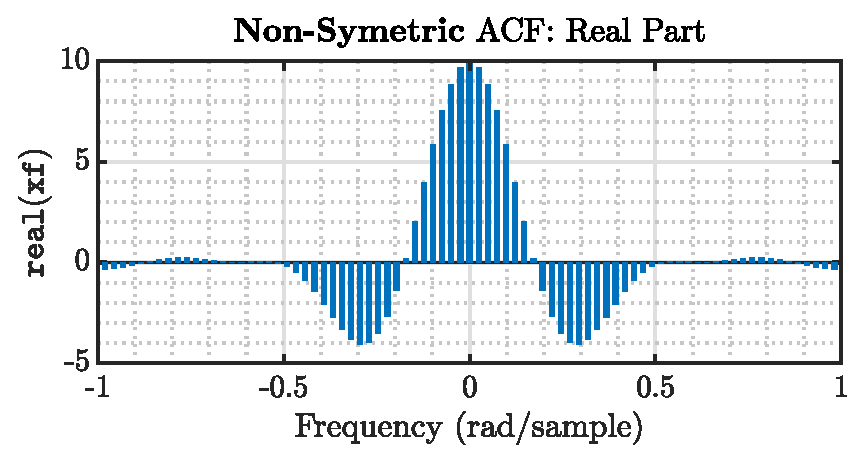
\includegraphics[height=1.5in]{report/spectrum-estimation/properties-of-power-spectral-density/assets/c/non_symetric_real-M_10}
    \end{subfigure}
    ~ 
    \begin{subfigure}{0.49\textwidth}
        \centering
        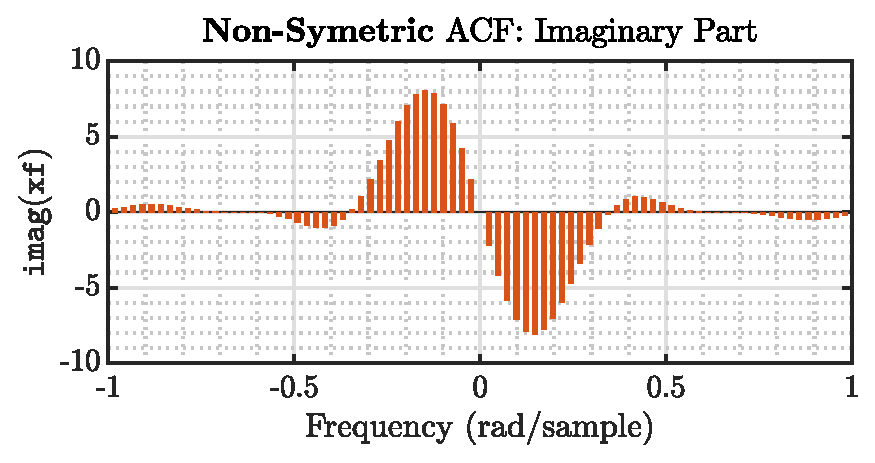
\includegraphics[height=1.5in]{report/spectrum-estimation/properties-of-power-spectral-density/assets/c/non_symetric_imag-M_10}
    \end{subfigure}
    \caption{Non-Symmetric $r_{xx}(k)$: real and imaginary parts of $P(w)$.}
    \label{fig:1_2_c_1}
\end{figure}

\begin{figure}[h]
    \centering
    \begin{subfigure}{0.49\textwidth}
        \centering
        \includegraphics[height=1.5in]{report/spectrum-estimation/properties-of-power-spectral-density/assets/c/comparison-M_10}
    \end{subfigure}
    ~
    \begin{subfigure}{0.49\textwidth}
        \centering
        \includegraphics[height=1.5in]{report/spectrum-estimation/properties-of-power-spectral-density/assets/c/comparison-M_128}
    \end{subfigure}
    \caption{Non-Symmetric $r_{xx}(k)$: $P(w)$ estimate using \texttt{abs} and \texttt{real}.}
    \label{fig:1_2_c_2}
\end{figure}


%% d)
\item

The figures in all the parts are generated, having previously centered the frequency axis via \texttt{fftshift}. Moreover, the signal length
is important when the frequency index, $w$, or the time index, $n$, are generated. Table \ref{tab:1_2_d} summarized the MATLAB commands
used for any case.

\begin{table}[h]
\centering
\begin{tabular}{|c||c|c|}
\hline
\textbf{Vector Length}, $L$ &
\textbf{Frequency Index}, $w$ &
\textbf{Time Index}, $n$ \\
\hline
\hline
\textbf{Even} &
$-\pi : \frac{2\pi}{L} : \pi - \frac{2\pi}{L}$ &
$-\frac{L}{2} : 1 : \frac{L}{2} - 1$ \\
\hline
\textbf{Odd} &
$-\pi + \frac{\pi}{L} : \frac{2\pi}{L - 1} : \pi - \frac{\pi}{L}$ &
$-\frac{L-1}{2} : 1 : \frac{L-1}{2} - 1$ \\
\hline
\end{tabular}
\caption{MATLAB commands for frequency $w$ and time $n$ indexes.}
\label{tab:1_2_d}
\end{table}

%
\end{enumerate}